\section{Results}
\label{sec:results}

\begin{figure}
\centering
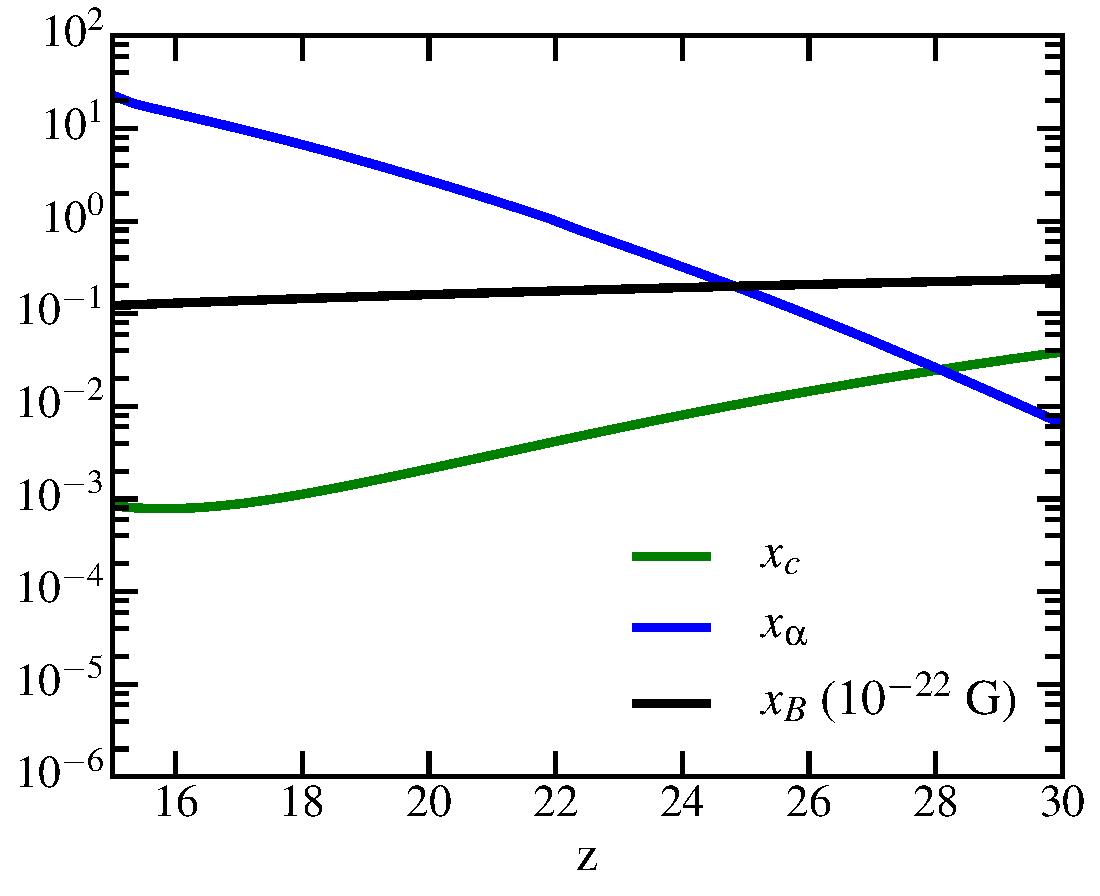
\includegraphics[width=.35\textwidth,keepaspectratio=true]{xs.pdf}
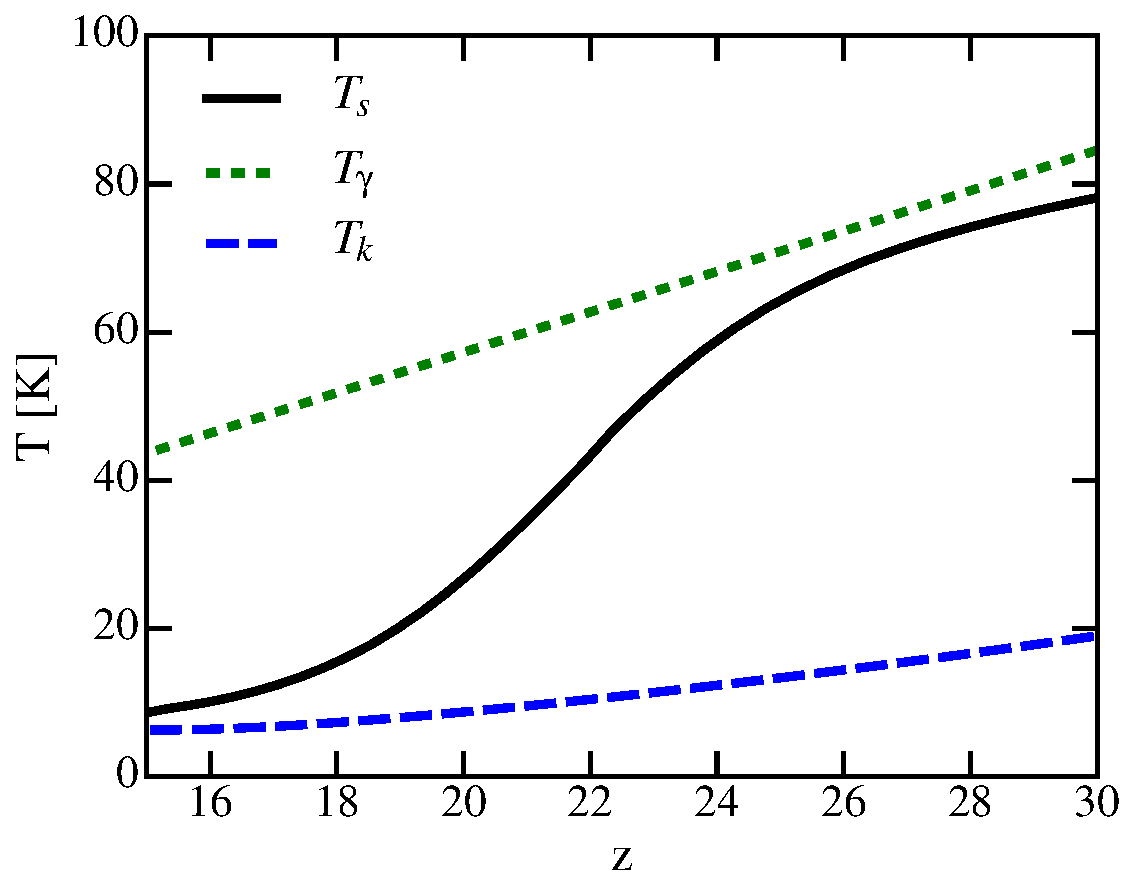
\includegraphics[width=.35\textwidth,keepaspectratio=true]{Ts.pdf}
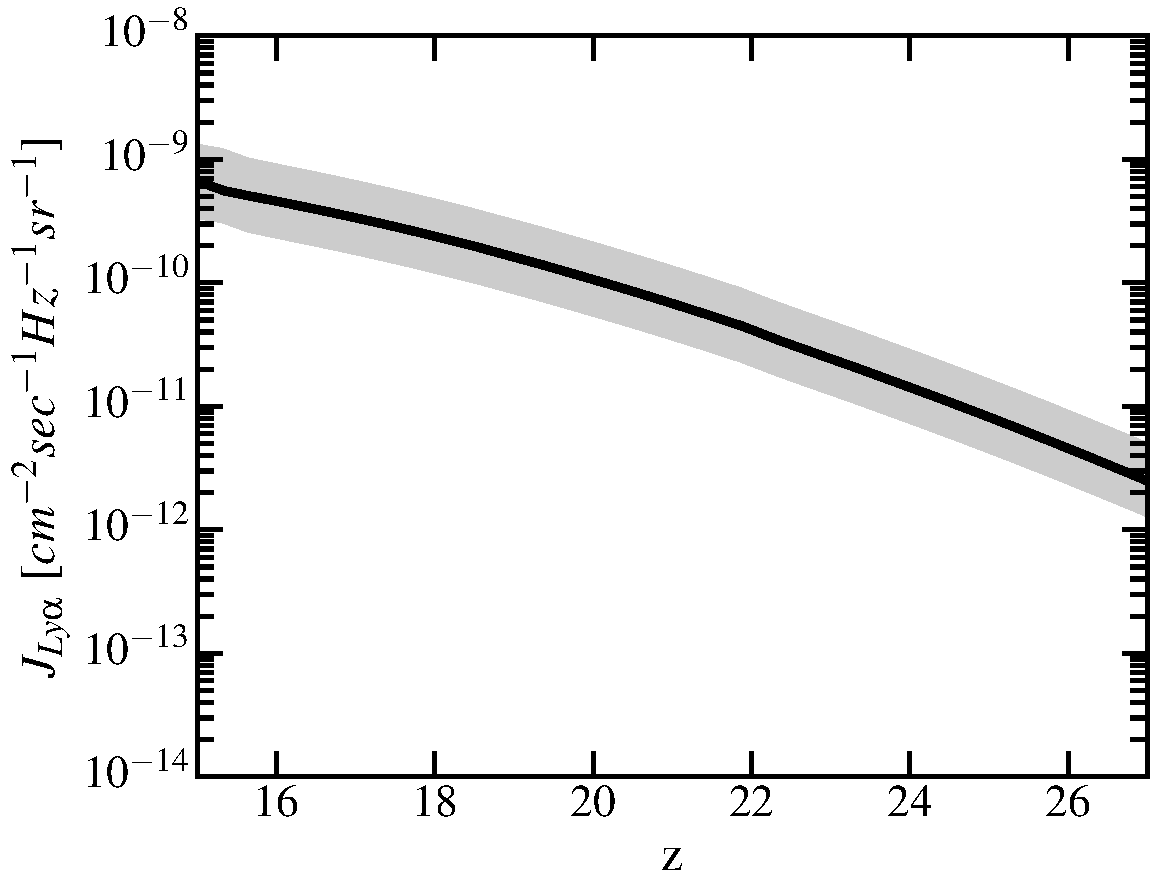
\includegraphics[width=.35\textwidth,keepaspectratio=true]{Jlya.pdf}
\caption{Inputs for sensitivity calculations: Lyman-$\alpha$ flux model, and the relevant spin- and kinetic- temperature models. \label{fig:cosmo}}
\end{figure}
We now proceede to numerically evaluate the sensitivity of a tomographic 21-cm survey to detecting magnetic fields during the pre-reionization epoch, using the formalism of previous two Sections. For the purposes of deriving numerical results, we only focus on one type of experimental setup---an array of closely-packed dipole antennas, such as the FFTT considered in \S\ref{subsec:uv}. The motivation for this choice is the fact that such configuration is known to maximize sensitivity of measurements based on the 2-point statistics \cite{2009PhRvD..79h3530T}, such as the one we propose in this work. For the parameters of this survey, we assume that a surface area of $(\Delta L\text{ km})^2$ is covered in dipole antennas, and that the experiment observes $\Omega_\text{survey}=1$sr of the sky for about 5 years.\footnote{The value used to evaluate Fisher formulas is actually 2 years. When corrected for the effect of Earth's rotation, and the fact that a given sky patch is above the horizon for only a fraction of a day, the effective observation time of 2 years translates to a (factor-of-a-few) longer wall-clock time.} For the sky temperature that enters the calculation of the noise power spectrum in \eq{\ref{eq:Pnoise_K}}, we assume a simple model of Galactic foregrounds from \cite{2008PhRvD..78b3529M}, where
\beq
T_\text{sky}  = 60\left(\frac{21}{100} (1+z)\right)^{2.55}\text{   [K]}.
\label{eq:tsys}
\eeq
Furthermore, we assume that the redshift range covered by the survey is $z\in[15,35]$.  Other ingredients entering the sensitivity calculation are the Lyman-$\alpha$ flux $J_{\text{Ly}\alpha}(z)$, and the spin and kinetic temperatures of the IGM; these are obtained using \texttt{21CMFAST} \cite{2011MNRAS.411..955M}, for standard cosmology, and are shown in Figure \ref{fig:cosmo}. We checked that the variation in the x-ray heating rate within a factor of a few from the fiducial model does not make significant changes to the presented results.
%more on heating; more on cosmo params; more on tobs being actually larger.

\begin{figure}
\centering
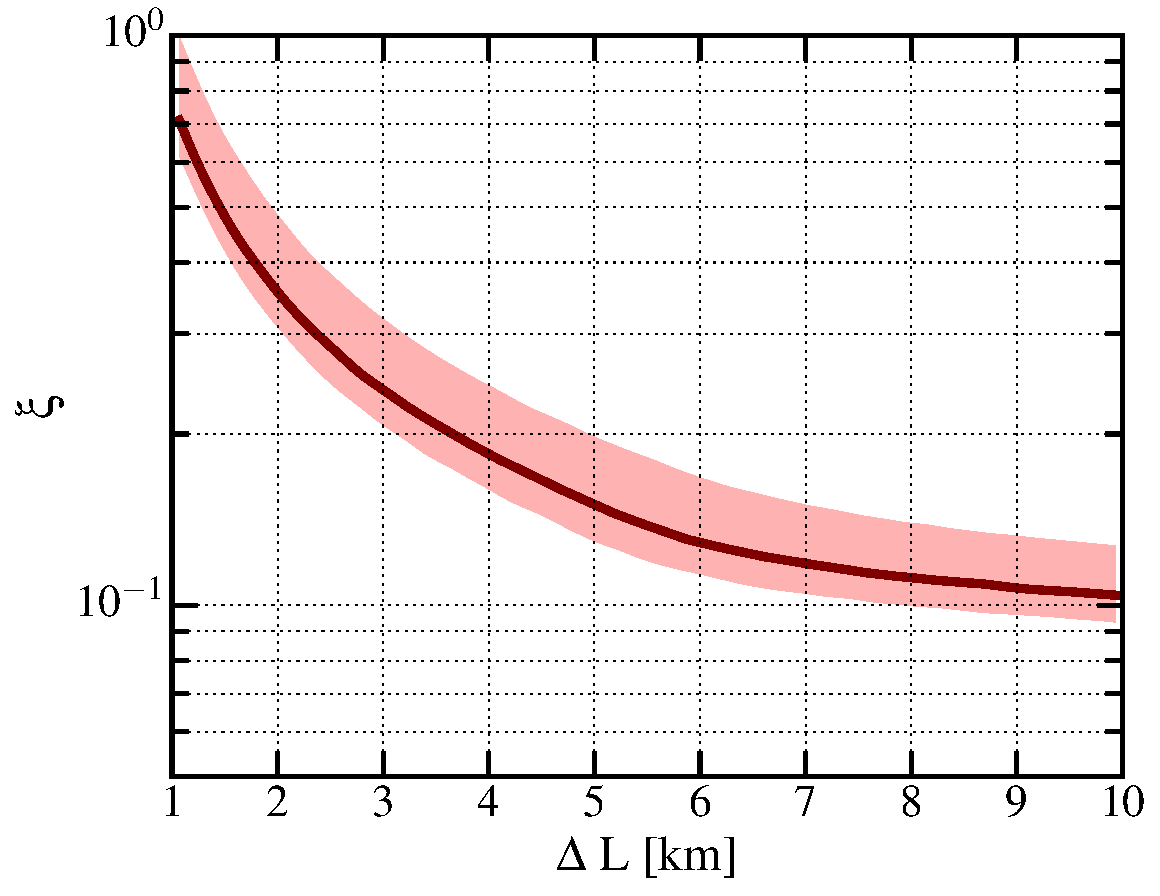
\includegraphics[width=.35\textwidth,keepaspectratio=true]{xi_vs_deltas.pdf}
\caption{FFTT sensitivity to distinguishing saturated case from no magnetic field (upper panel), as a function of maximum array baseline, assuming a survey size of 1 sr, for survey duration of 2 years.\label{fig:xi_vs_deltas}}
\end{figure}
\begin{figure}
\centering
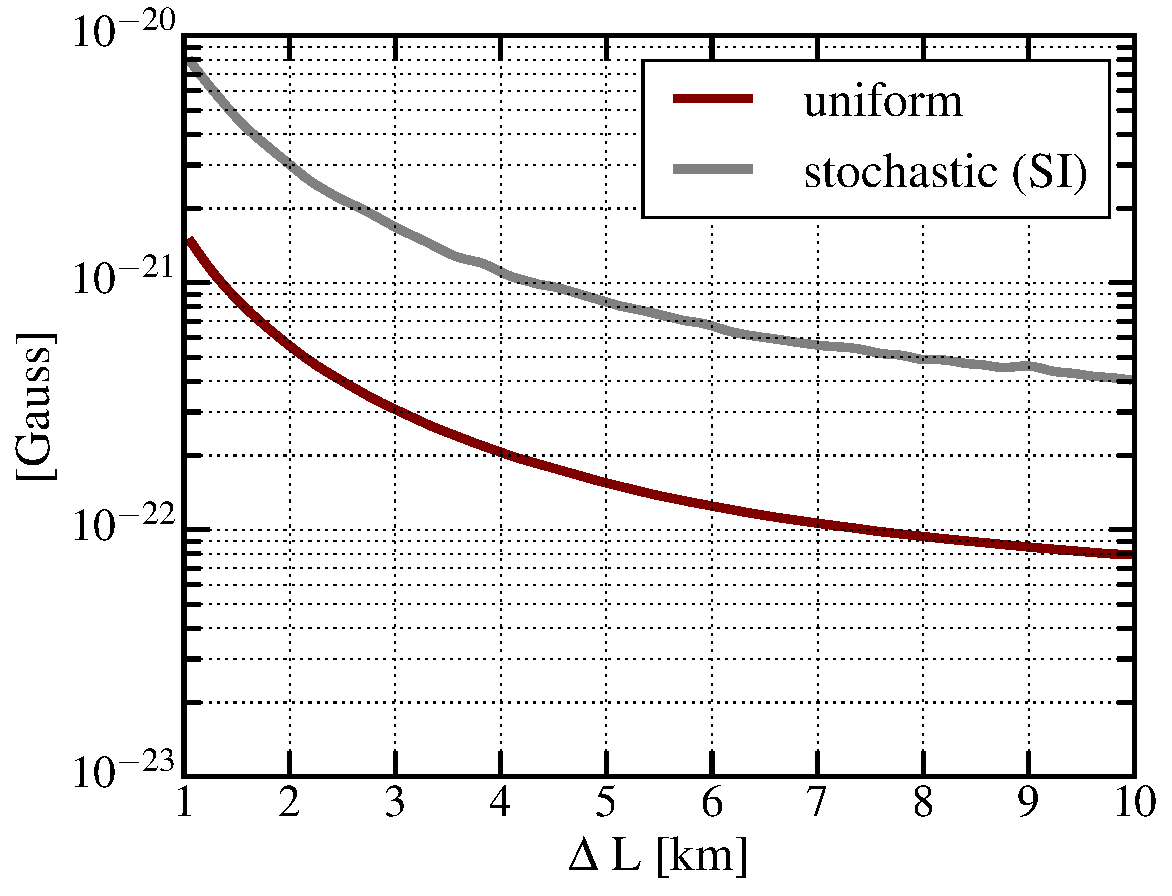
\includegraphics[width=.35\textwidth,keepaspectratio=true]{B_vs_deltas.pdf}
\caption{FFTT sensitivity to detecting a uniform and stochastic magnetic field (stochastic field is assumed to have a scale-independent (SI) power spectrum, and shown is the rms per $log K$, $A_0/\pi$.), as a function of maximum array baseline, assuming a survey size of 1 sr, for survey duration of 2 years.\label{fig:B_vs_deltas}}
\end{figure}
Figures \ref{fig:xi_vs_deltas} and \ref{fig:B_vs_deltas} show how the sensitivity changes as a function of the maximum baseline $\Delta L$ (since different baselines may correspond to different stages of the experiment). Figure \ref{fig:xi_vs_deltas} shows $1\sigma$ sensitivity to measuring parameter $\xi$ of \eq{\ref{eq:saturated_P}}, that distinguishes amongst the zero magnetic field case and the case where the field is strong enough that the signal saturates (in the sense described in \S\ref{sec:method}). This parameter is by definition boud between the values of 0 and 1, where 0 represents the case of no magnetic field, and 1 represents the saturated case. From this Figure, we can see that, for example, a little over a square kilometer of covarega area is necessary for a $1\sigma$ detection of magnetic fields stronger than about $10^{-21}$ Gauss comoving. While this size of a radio array is still futuristic in terms of the shear number of antennas (compare to the SKA \cite{2008arXiv0802.1727C}, for example), the number of mode measurements required for this measurement corresponds to the computational demands for the next-generation 21-cm cosmology experiment, and may thus be feasible in the coming couple of decades. 

Figure \ref{fig:B_vs_deltas} is obtained by evaluating the expressions of Eqs.~(\ref{eq:fisher_patch}) and (\ref{eq:snr_ints}), and shows sensitivity to measuring the scaled value of the magnetic field in the case of a uniform field (dark red line), and the sensitivity to measuring the amplitude of a particular model for a stochastic field (gray line)---the scale-independent (SI) power spectrum discussed in \S\ref{sec:fisher}. While the numerical calculation behind this plot assumed that the brightness temperature is a linear function of the field strength, this assumption is not guaranteed to hold---it breaks in the saturation limit, as discussed in \S\ref{sec:method}. In order to understand how the constraints (or, sensitivities) of Figure \ref{fig:B_vs_deltas} compare to the saturation ``ceiling'' at the redshifts we integrate over, we present a rough calculation of the saturation as a function of redshift, and compare it to the values of the $z$-dependent integrands of \eq{\ref{eq:fisher_patch}}. From this Figure, we can see that only above the coverage of about $16$km$^2$ are we able to actually measure the exact value of the amplitude of the magnetic field power spectrum.
\begin{figure}
\centering
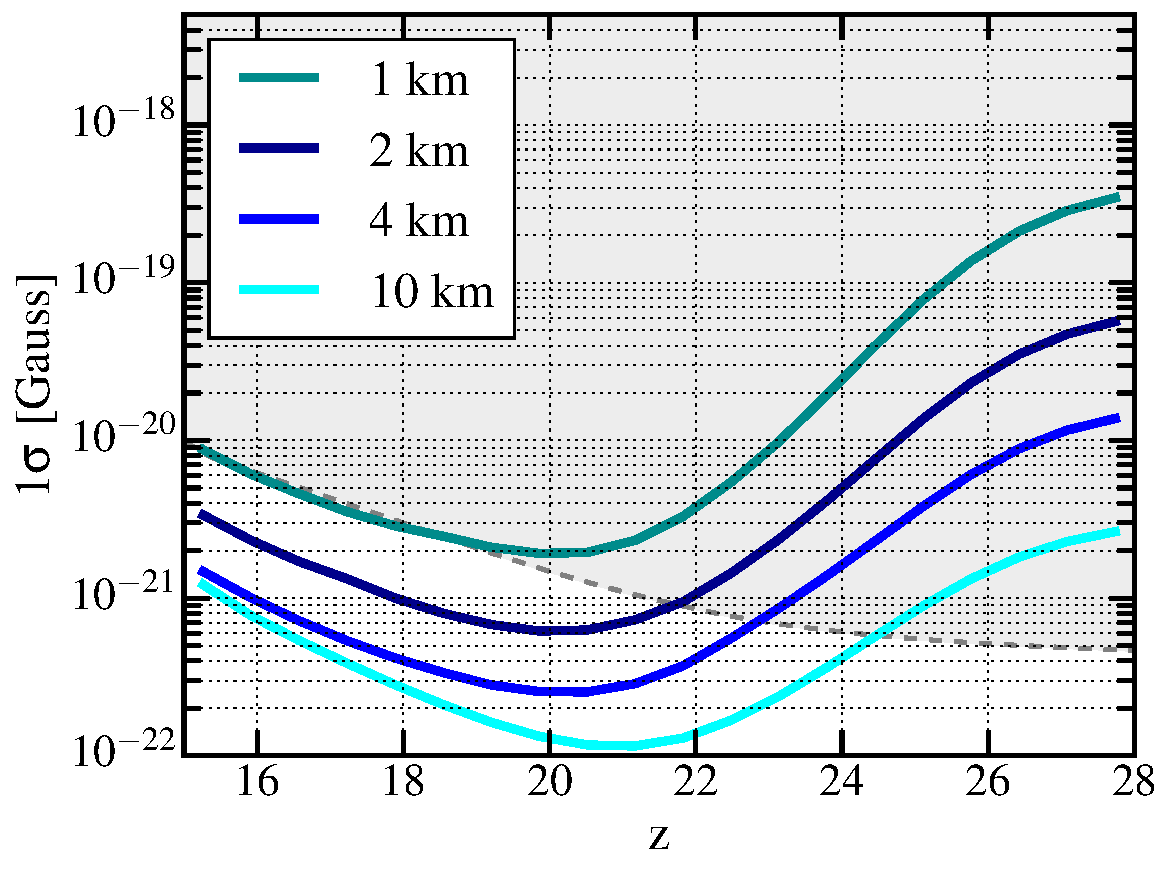
\includegraphics[width=.35\textwidth,keepaspectratio=true]{sigmaB0_vs_z.pdf}
\caption{Saturation ceiling is shown as a shaded gray area, and integrand of \eq{\ref{eq:fisher_patch}} (inverse sqare root of it) is shown as a function of redshift, for several maximum baseline sizes.  When the colored curves are below the saturation limit around their minima, the analysis assuming unsaturated regime is valid.\label{fig:Bsat}}
\end{figure}
